% 
% NIT Patna Resume Template v2.1
% Author: Pavan Kumar Dubasi
% NIT Patna - IMSc., Mathematics (2019-24)
% LinkedIn: https://www.linkedin.com/in/im-pavankumar/
% 


\documentclass[a4paper,11pt]{article}

% Package imports

\usepackage{latexsym}
\usepackage{xcolor}
\usepackage{float}
\usepackage{ragged2e}
\usepackage[empty]{fullpage}
\usepackage{wrapfig}
\usepackage{tabularx}
\usepackage{titlesec}
\usepackage{array}  
\usepackage{multirow}  
\usepackage{geometry}
\usepackage{marvosym}
\usepackage{verbatim}
\usepackage{enumitem}
\usepackage{fancyhdr}
\usepackage{multicol}
\usepackage{graphicx}
\usepackage{cfr-lm}
\usepackage[T1]{fontenc}
\usepackage{fontawesome5}
\usepackage[hidelinks]{hyperref} 
\usepackage{pdfcomment}
\usepackage{microtype}
\usepackage{tabularx} % Required for tables that stretch to page width
\usepackage{array} % Required for vertical centering in tables
% Color definitions
\definecolor{darkblue}{RGB}{0,0,139}

% Page layout
\geometry{left=1.2cm, top=0.58cm, right=1.2cm, bottom=1cm}
\setlength{\multicolsep}{0pt} 
\pagestyle{fancy}
\fancyhf{} % clear all header and footer fields
\fancyfoot{}
\renewcommand{\headrulewidth}{0pt}
\renewcommand{\footrulewidth}{0pt}
\setlength{\footskip}{4.08pt}

% Hyperlink setup
\hypersetup{
    colorlinks=true,
    linkcolor=darkblue,
    filecolor=darkblue,
    urlcolor=darkblue,
}

% Custom box settings
\usepackage[most]{tcolorbox}
\tcbset{
    frame code={},
    center title,
    left=0pt,
    right=0pt,
    top=0pt,
    bottom=0pt,
    colback=gray!20,
    colframe=white,
    width=\dimexpr\textwidth\relax,
    enlarge left by=-2mm,
    boxsep=4pt,
    arc=0pt,outer arc=0pt,
}

% URL style
\urlstyle{same}

% Text alignment
\raggedright
\justifying

\setlength{\tabcolsep}{0in}

% Section formatting
\titleformat{\section}{
  \vspace{-4pt}\scshape\raggedright\large\bfseries
}{}{0em}{}[\color{black}\titlerule \vspace{-7pt}]

% Custom commands
\newcommand{\resumeItem}[2]{
  \item{
    \textbf{#1}{\hspace{0.5mm}#2 \vspace{-0.5mm}}
  }
}

\newcommand{\resumePOR}[3]{
\vspace{0.5mm}\item
    \begin{tabular*}{0.97\textwidth}[t]{l@{\extracolsep{\fill}}r}
        \textbf{#1}\hspace{0.3mm}#2 & \textit{\small{#3}} 
    \end{tabular*}
    \vspace{-2mm}
}

\newcommand{\resumeSubheading}[4]{
\vspace{0.5mm}\item
    \begin{tabular*}{0.98\textwidth}[t]{l@{\extracolsep{\fill}}r}
        \textbf{#1} & \textit{\footnotesize{#4}} \\
        \textit{\footnotesize{#3}} &  \footnotesize{#2}\\
    \end{tabular*}
    \vspace{-2.4mm}
}

% \newcommand{\resumeProject}[4]{
% \vspace{0.5mm}\item
%     \begin{tabular*}{0.98\textwidth}[t]{l@{\extracolsep{\fill}}r}
%         \textbf{#1} & \textit{\footnotesize{#3}} \\
%         \footnotesize{\textit{#2}} & \footnotesize{#4}
%     \end{tabular*}
%     \vspace{-2.4mm}
% }
\newcommand{\resumeProject}[4]{
\vspace{0.5mm}\item
    \begin{tabular*}{0.98\textwidth}[t]{l@{\extracolsep{\fill}}r}
        \textbf{#1}\hspace{0.5em}#4 & \textit{\footnotesize{#3}} \\
    \end{tabular*}
    \vspace{-2.4mm}
}

\newcommand{\resumeSubItem}[2]{\resumeItem{#1}{#2}\vspace{-4pt}}

\renewcommand{\labelitemi}{$\vcenter{\hbox{\tiny$\bullet$}}$}
\renewcommand{\labelitemii}{$\vcenter{\hbox{\tiny$\circ$}}$}

\newcommand{\resumeSubHeadingListStart}{\begin{itemize}[leftmargin=*,labelsep=1mm]}
\newcommand{\resumeHeadingSkillStart}{\begin{itemize}[leftmargin=*,itemsep=1.7mm, rightmargin=2ex]}
\newcommand{\resumeItemListStart}{\begin{itemize}[leftmargin=*,labelsep=1mm,itemsep=0.5mm]}

\newcommand{\resumeSubHeadingListEnd}{\end{itemize}\vspace{2mm}}
\newcommand{\resumeHeadingSkillEnd}{\end{itemize}\vspace{-2mm}}
\newcommand{\resumeItemListEnd}{\end{itemize}\vspace{-2mm}}
\newcommand{\cvsection}[1]{%
\vspace{2mm}
\begin{tcolorbox}
    \textbf{\large #1}
\end{tcolorbox}
    \vspace{-4mm}
}

\newcolumntype{L}{>{\raggedright\arraybackslash}X}%
\newcolumntype{R}{>{\raggedleft\arraybackslash}X}%
\newcolumntype{C}{>{\centering\arraybackslash}X}%

% Commands for icon sizing and positioning
\newcommand{\socialicon}[1]{\raisebox{-0.05em}{\resizebox{!}{1em}{#1}}}
\newcommand{\ieeeicon}[1]{\raisebox{-0.3em}{\resizebox{!}{1.3em}{#1}}}

% Font options
\newcommand{\headerfonti}{\fontfamily{phv}\selectfont} % Helvetica-like (similar to Arial/Calibri)
\newcommand{\headerfontii}{\fontfamily{ptm}\selectfont} % Times-like (similar to Times New Roman)
\newcommand{\headerfontiii}{\fontfamily{ppl}\selectfont} % Palatino (elegant serif)
\newcommand{\headerfontiv}{\fontfamily{pbk}\selectfont} % Bookman (readable serif)
\newcommand{\headerfontv}{\fontfamily{pag}\selectfont} % Avant Garde-like (similar to Trebuchet MS)
\newcommand{\headerfontvi}{\fontfamily{cmss}\selectfont} % Computer Modern Sans Serif
\newcommand{\headerfontvii}{\fontfamily{qhv}\selectfont} % Quasi-Helvetica (another Arial/Calibri alternative)
\newcommand{\headerfontviii}{\fontfamily{qpl}\selectfont} % Quasi-Palatino (another elegant serif option)
\newcommand{\headerfontix}{\fontfamily{qtm}\selectfont} % Quasi-Times (another Times New Roman alternative)
\newcommand{\headerfontx}{\fontfamily{bch}\selectfont} % Charter (clean serif font)

% Define personal information
\newcommand{\name}{Mahbod Tajdini} % Your Name
\newcommand{\course}{Master of Science} % Your Course
\newcommand{\roll}{XXXXXX} % Your Roll No.
\newcommand{\phone}{xxxxxxxxxx} % Your Phone Number
\newcommand{\emaila}{personalmail@email.com} % Email 1
\newcommand{\emailb}{mahbodtajdini@gmail.com} % Email 2
\newcommand{\github}{username} % Github
\newcommand{\website}{https://example.com/} % Website
\newcommand{\linkedin}{linkedinuser} % LinkedIn
% ==== Add these custom commands/macros with your other \newcommand's ====
% Compact, no-bullet list for publications
\newenvironment{publist}{
  \begin{itemize}[leftmargin=*,labelsep=0mm,itemsep=0.6mm,topsep=0.2mm]
  \renewcommand\labelitemi{} % no bullet
}{
  \end{itemize}\vspace{-2mm}
}

% Small, consistent link style for DOI / arXiv / Code
\newcommand{\publink}[2]{[\href{#2}{\textcolor{darkblue}{#1}}]}

% One-line builder: Title (bold) on the left; venue+date (italic) on the right;
% authors on the next line; links on the third line. Uses your tabularx look.
\newcommand{\publicationEntry}[5]{%
\vspace{0.5mm}\item
  \begin{tabularx}{0.98\textwidth}[t]{@{}L R@{}}
    \textbf{#1} & \textit{\footnotesize #3} \\
    \multicolumn{2}{@{}l@{}}{\footnotesize\textit{#2}} \\
    \multicolumn{2}{@{}l@{}}{\footnotesize #4\hspace{0.8em}#5} \\
  \end{tabularx}
\vspace{-2.0mm}
}
% Args:
%  #1 Title
%  #2 Authors (e.g., Mahbod Tajdini, …)
%  #3 Venue + Month Year (or “Under Review – Venue”)
%  #4 Left links (e.g., \publink{DOI}{...} \publink{arXiv}{...})
%  #5 Right links (e.g., \publink{\faGithub}{...}) — leave empty if none

\begin{document}
\fontfamily{cmr}\selectfont

%----------HEADING-----------------
% \parbox{2.35cm}{%
% \includegraphics[width=2cm,clip]{pic2.jpg}
% }
% \parbox{\dimexpr\linewidth-2.8cm\relax}{
% \begin{tabularx}{\linewidth}{L r}
%   \textbf{\LARGE \name} & \faIcon{phone} +41-784478887 \\
%   \course & \faIcon{envelope-square} \href{mailto:mahbodtajdini@gmail.com}{\emailb} \\
%   in Data Science  & \faIcon{linkedin} \href{https://www.linkedin.com/in/mahbodtajdini/}{LinkedIn} \\
%   UZH and ETH Zürich, Switzerland
%   & \faIcon{github} \href{https://github.com/Ace3Z}{GitHub} 
% \end{tabularx}
% }
\parbox{2.15cm}{%
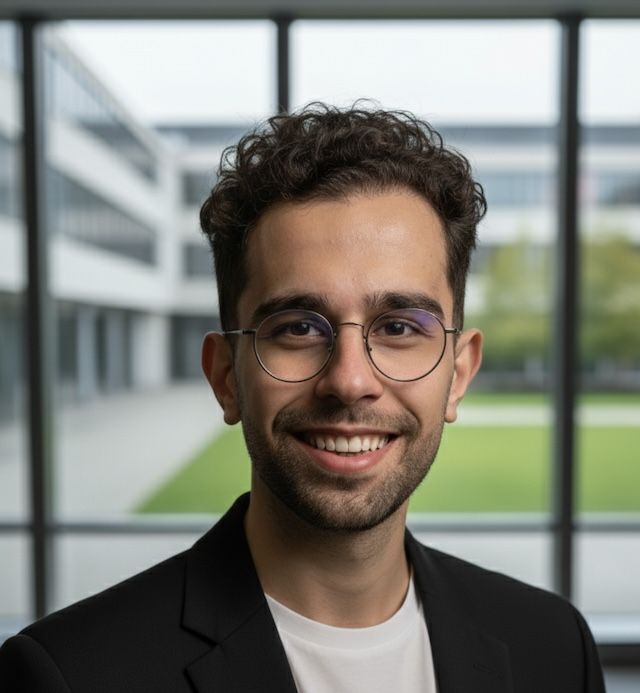
\includegraphics[width=2cm,clip]{pic.jpg}
}
\parbox{\dimexpr\linewidth-2.8cm\relax}{
\begin{tabularx}{\linewidth}{L r}
  \textbf{\LARGE \name} & \faIcon{phone} +41-784478887 \\

  Master of Science in Data Science
  & \faIcon{envelope-square} \href{mailto:mahbodtajdini@gmail.com}{\emailb} \\

  UZH and ETH Zürich, Switzerland
  &
  \faIcon{globe} \href{https://mahbodtajdini.com/}{Portfolio}
  \,|\, 
  \faIcon{linkedin} \href{https://www.linkedin.com/in/mahbodtajdini/}{LinkedIn}
  \,|\, 
  \faIcon{github} \href{https://github.com/Ace3Z}{GitHub}
\end{tabularx}
}


\vspace{-2mm}

% \section{\textbf{Education}}
% \vspace{1mm}
% \setlength{\tabcolsep}{5pt}
% \begin{tabularx}{\textwidth}{|>{\centering\arraybackslash}X|>{\centering\arraybackslash}p{8cm}|>{\centering\arraybackslash}p{3cm}|>{\centering\arraybackslash}p{2.5cm}|}
%   \hline
%   \textbf{Degree} & \textbf{Institute} & \textbf{GPA} & \textbf{Year} \\
%   \hline
%   MSc in Data Science & National Institute of Technology, Patna & N/A (Ongoing) & 2025-Present \\ 
%   \hline
%   BSc in Artificial Intelligence & Vrije Universiteit Amsterdam (VU Amsterdam)
%  & 8.5/10 (=4.0 GPA) & 2022-2025 \\
%   \hline
%   International Baccalaureate Diploma Programme (IBDP) & Tehran International School & 41/45 & 2020-2022 \\
%   \hline
% \end{tabularx}
% \vspace{-4mm}


\section{\textbf{Education}}
\vspace{1mm}
\setlength{\tabcolsep}{5pt}
\begin{tabularx}{\textwidth}{|>{\centering\arraybackslash}m{4.5cm}|>{\centering\arraybackslash}m{6.84cm}|>{\centering\arraybackslash}X|>{\centering\arraybackslash}m{2.5cm}|}
\hline
\textbf{Degree} & \textbf{Institute} & \textbf{CGPA} & \textbf{Year} \\
\hline

\multirow{2}{*}{\textbf{MSc in Data Science}} & Universität Zürich (UZH) & \multirow{2}{*}{N/A (Ongoing)} & \multirow{2}{*}{2025 - Present} \\
\cline{2-2}
& ETH Zürich (Special Student) & & \\
\hline

\textbf{BSc in Artificial} & Vrije Universiteit Amsterdam & \multirow{2}{*}{8.5/10 (=4.0 GPA)} & \multirow{2}{*}{2022 - 2025} \\
\textbf{Intelligence} & (VU Amsterdam) & & \\
% \hline
% The Thesis Row (Spanning all 4 columns)
\multicolumn{4}{|p{0.95\textwidth}|}{
\centering \small \textbf{Bachelor's Thesis:} \textit{Exploring Ball Recovery Times in Professional
Football: Insights and Patterns} \hfill 
} \\ \hline
% \textbf{BSc in Artificial Intelligence} & Vrije Universiteit Amsterdam \newline (VU Amsterdam) & 8.5/10 (=4.0 GPA) & 2022 - 2025 \\
% \hline
\end{tabularx}
\vspace{-4mm}

\section{\textbf{Research Experience}}
\vspace{-0.4mm}
\resumeSubHeadingListStart
\resumeSubheading
    {ETH Zürich - Computer Vision and Geometry Group (CVG) [\href{https://cvg.ethz.ch/}{\faIcon{globe}}]}{Zürich, Switzerland}
    {Graduate Student Researcher}{Mar 2026 – Present}
    \resumeItemListStart
      \item Working on state-of-the-art dynamic SLAM under Dániel Béla Baráth at the Computer Vision and Geometry Group, focusing on integrating semantic scene graphs into deep visual SLAM by extending DROID-SLAM in the Wild (DROID-W) to improve efficiency and robustness in unconstrained environments
    \resumeItemListEnd

\resumeSubheading
    {ETH Zürich - Ecosystem and Landscape Evolution Group (ELE) [\href{https://ele.ethz.ch/}{\faIcon{globe}}]}{Zürich, Switzerland}
    {Research Assistant}{Mar 2026 – Present}
    \resumeItemListStart
      \item Supporting the development of \href{https://wildinsync.org/}{WildInSync}, an open platform for integrating ecological monitoring data to advance biodiversity research and conservation efforts
    \resumeItemListEnd
\resumeSubheading
    {EPFL - Signal Processing Laboratory (LTS4) [\href{https://www.epfl.ch/labs/lts4/}{\faIcon{globe}}]}{Lausanne, Switzerland}
    {Visiting Student Researcher}{Feb 2026 – Present}
    \resumeItemListStart
      \item Conducting research on scalable cell-graph representations for digital pathology, focusing on batch-effect–robust graph construction, edge enhancement with tissue context, and graph diversity to improve generalization
    \item Investigating multimodal foundation-model approaches that combine cell graphs and vision models, exploring efficient fine-tuning strategies and curated large-scale datasets for robust zero-shot and transfer learning
    \resumeItemListEnd
    
    % \resumeSubheading 
    % {ETH Robotics Club 
    % [\href{https://www.ethrobotics.ch/}{\faIcon{globe}}]}{Zürich, Switzerland}
    % {Robotic Perception Engineer}{Feb 2026 – Mar 2026}
    % \resumeItemListStart
    %   \item Conducting research and applied development on perception and computer vision systems for \textit{Gibby}, a tree-climbing research robot. The vision stack supports environment perception, branch and terrain understanding, localization, and autonomous navigation in complex, unstructured forest environments
    % \resumeItemListEnd

\resumeSubheading 
    {VU Amsterdam - Sports Intelligence Lab [\href{https://sportsintelligencelab.com/}{\faIcon{globe}}]}{Remote}
    {Research Assistant}{Jun 2025 – Mar 2026}
    \resumeItemListStart
      \item Conducting data-driven research on ball recovery in professional football and exploring machine learning applications in the sport under the supervision of Dr. Mauricio Verano Merino
    \item Analyzed large-scale educational data to evaluate the effects of Generative AI tools on student outcomes in programming courses, contributing to a paper accepted at \emph{ICSE 2026}
    \resumeItemListEnd


\resumeSubheading
    {Forward Football [\href{https://forward.football/} {\faIcon{globe}}]}{Amsterdam, Netherlands}
    {AI Research Intern}{Sep 2024 – Jun 2025}
    \resumeItemListStart
    %   \item Researched team formation and strategic optimization in professional football through advanced ML and AI methodologies
    % \item Analyzed large-scale spatiotemporal datasets to model player interactions, quantify team performance, and derive data-driven tactical insights
     \item Researched machine learning and computer vision models for football intelligence and tactical optimization
     \item Analyzed large-scale spatiotemporal datasets to model player interactions, quantify team performance, and derive data-driven tactical insights
% • Built machine learning and computer vision models for football intelligence and tactical optimization
% • Performed large-scale data science analysis on spatiotemporal sports datasets
% • Developed deep learning pipelines for player tracking, performance modeling, and tactical insights
    \resumeItemListEnd
\resumeSubHeadingListEnd
\vspace{-8mm}




\section{\textbf{Work Experience}}
\vspace{-0.4mm}
\resumeSubHeadingListStart
\resumeSubheading
  {ETH Zürich - Ecosystem and Landscape Evolution Group (ELE)
  [\href{https://www.vvz.ethz.ch/Vorlesungsverzeichnis/lerneinheit.view?semkez=2026S\&ansicht=ALLE\&lerneinheitId=201478\&lang=en}{\faIcon{globe}}]}
  {Zürich, Switzerland}
    {Teaching Assistant}{Jan 2026 – Present}
    \resumeItemListStart
      \item Serving as a Teaching Assistant for Environmental Systems Data Science: Machine Learning (701-3003-00L) under the supervision of Prof. Dr. Loïc Pellissier and Dr. Camille Pierre Albouy
    \resumeItemListEnd

\resumeSubheading
  {Forward·Inc
  [\href{https://www.newcomersforward.com/get-involved/}{\faIcon{globe}}]}
  {Amsterdam, Netherlands}
    {Student AI Consultant}{Jan 2026 – Mar 2026}
    \resumeItemListStart
      \item Advising mission-driven organization on AI implementation through research and data analysis, evaluating AI tools and platforms, and delivering strategic roadmaps that align AI adoption with organizational goals and operational improvements
    \resumeItemListEnd
    \newpage



\resumeSubheading
    {Universität Zürich - IFI [\href{https://www.ifi.uzh.ch/en/seal/teaching/courses/info1.html}{\faIcon{globe}}]}{Zürich, Switzerland}
    {Head Teaching Assistant}{Sep 2025 – Dec 2025}
    \resumeItemListStart
      \item Served as Head Teaching Assistant (TA) for Informatics I (22AINF02) under the supervision of Prof. Dr. Harald Gall and Dr. Carol Alexandru, leading the TA team and managing teaching operations, exercise design, and assessment processes to ensure high-quality student learning support and effective course delivery
    \resumeItemListEnd
% \newpage

\resumeSubheading
    {VU Amsterdam - Faculty of Science [\href{https://vu.nl/en}{\faIcon{globe}}]}{Amsterdam, Netherlands}
    {Teaching Assistant}{Apr 2023 - Jun 2025}
    \resumeItemListStart
      \item Mentored new TAs through workshops, training sessions, and personalized feedback as a TA Mentor, enhancing instructional quality across the Faculty of Science
        \item Taught and supported Machine Learning–focused courses and labs across 10+ undergraduate and Honors-level courses %\footnote{Courses assisted: Introduction to Python Programming (2023, 2024); Computational Thinking (2023, 2024); The Impact of Algorithms on Human Lives – Honors course (2024); Project Intelligent Systems (2024); Dynamic Modelling (2024); Human-Computer Interaction for AI (2024, 2025); Applied Programming (2024, 2025); Machine Learning (2024); Project Conversational Agents (2025).}

      \item Coordinated TA activities, contributed to course design, and facilitated communication between instructors and students as Head TA for the course: Computational Thinking (X\_400475)

    \resumeItemListEnd
\resumeSubheading
    {Baridsoft [\href{https://baridsoft.net/} {\faIcon{globe}}]}{Tehran, Iran}
    {Information Technology Intern }{Jun 2021 – Aug 2021}
    \resumeItemListStart
      \item Worked on computer systems, network infrastructure, and IT support, with hands-on experience in troubleshooting, device configuration, and maintaining internal systems

    \resumeItemListEnd


\resumeSubHeadingListEnd
\vspace{-8mm}

% \section{\textbf{Projects}}
% \vspace{-0.4mm}
% \resumeSubHeadingListStart

% \resumeProject
%     {Project A: [Brief Description]}
%     {Tools: [List of tools and technologies used]}
%     {Month Year - Month Year}
%     {{}[\href{https://github.com/your-username/project-a}{\textcolor{darkblue}{\faGithub}}]}
% \resumeItemListStart
%     \item Developed [specific feature/system] for [specific purpose]
%     \item Implemented [specific technology] for [specific goal], achieving [specific result]
%     \item Created [specific component], ensuring [specific benefit]
%     \item Applied [specific method] to analyze [specific aspect]
% \resumeItemListEnd

% \resumeProject
%     {Project B: [Brief Description]}
%     {Tools: [List of tools and technologies used]}
%     {Month Year}
%     {{}[\href{https://github.com/your-username/project-b}{\textcolor{darkblue}{\faGithub}}]}
% \resumeItemListStart
%     \item Designed [specific component/tool] for [specific function]
%     \item Integrated [specific technology] to enhance [specific feature]
%     \item Evaluated [specific process] leading to [specific outcome]
%     \item Collaborated with [specific team/individual] on [specific aspect]
% \resumeItemListEnd
% \resumeSubHeadingListEnd
% \vspace{-8mm}



\section{\textbf{Research Publications}}
\vspace{-0.4mm}
\begin{publist}

% \publicationEntry
%   {Paper Title 1}
%   {Mahbod Tajdini, [Co-authors]}
%   {Proceedings of [Conference], [Month Year]}
%   {\publink{DOI}{https://doi.org/your-doi}\;\; \publink{arXiv}{https://arxiv.org/abs/your-id}}
%   {\publink{\faGithub}{https://github.com/your/repo}}

% \publicationEntry
%   {Paper Title 2}
%   {Mahbod Tajdini, [Co-authors]}
%   {Under Review – [Target Venue]}
%   {\publink{Preprint}{https://your-preprint-link}}
  {} % (no code link)

% Add more \publicationEntry blocks as needed
% \publicationEntry
%   {Exploring Ball Recovery Times in Professional Football: Insights and Patterns}
%   {\textbf{Mahbod Tajdini}, Mauricio Verano Merino}
%   {In preparation for submission to npj Artificial Intelligence 2026, Nature Collection “AI in Sports”}
%   {}{}
%   \vspace{-0.38cm}
\publicationEntry
  {Capitalising on Football Data with Machine Learning: A Literature Review}
  {Dionysios Kyriazopoulos, \textbf{Mahbod Tajdini}, Mauricio Verano Merino, }
  {Under Review - ACM Computing Surveys (ACM CSUR) 2026} %  In preparation for submission to ACM Computing Surveys (ACM CSUR) 2026
  
  {}{}
  \vspace{-0.38cm}

\publicationEntry
  {The Clash of Codes: From Peer-to-Peer Duplication to
AI-Generation in Introductory Programming Assignments}
  {Jose Maria Zuzarte Reis Claver$^{*}$, \textbf{Mahbod Tajdini$^{*}$}, Mauricio Verano Merino}
  {To Appear - ICSE 2026}
  {}{}
\vspace{-0.38cm}
\publicationEntry
  {Programming Lego MINDSTORMS Robots
using NI LabVIEW®}
  {Pooyan Nayyeri, \textbf{Mahbod Tajdini}}
{eBook - April 2022}
{\publink{open-access eBook}{https://pnnayyeri.github.io/contents/labview_book_en.pdf}}{}
\end{publist}
% \vspace{-2mm}


\section{\textbf{Positions of Responsibility}}
\vspace{-0.4mm}
\resumeSubHeadingListStart
    
    \resumePOR{\href{https://www.analytics-club.org/hack4good}{Hack4Good Organizing Staff}, } % Position
    {Analytics Club at ETH Zürich} %Club,Event
    {Nov 2025 – Present}
    \resumePOR{\href{https://www.studentrobotics.eu/}{Executive Staff}, } % Position
    {European Student Robotics Association (ESRA)} %Club,Event
    {Nov 2025 – Mar 2026}
    \resumePOR{\href{https://vu.nl/en/student/participation-in-decision-making/programme-committees}{Voting member of the Program Committee for AI}, } % Position
    {VU Amsterdam} %Club,Event
    {Oct 2022 – Jun 2025} %Tenure Period
    \resumePOR{\href{https://vu.nl/en/education/bachelor/artificial-intelligence}{Year Representative for BSc AI}, } % Position
    {VU Amsterdam} %Club,Event
    {Oct 2022 – Jun 2025} %Tenure Period
    \resumePOR{\href{https://www.linkedin.com/in/mahbodtajdini/details/experience/1707225648347/single-media-viewer/?profileId=ACoAADRMwb4Byod_U7xDS_8TfVrdUDd9eVLqE5k}{International Student Ambassador}, } % Position
    {VU Amsterdam} %Club,Event
    {Oct 2022 – Jun 2025} %Tenure Period
    \resumePOR{\href{https://wro-association.org/}{Robotics Competition Judge}, } % Position
    {WRO Netherlands} %Club,Event
    {Jun 2023 - Jul 2023} %Tenure Period

\resumePOR{\href{https://me.ut.ac.ir/introduction}{       Captain of the Student Robotics Team}, } % Position
    {University of Tehran} %Club,Event
    {Jun 2017 - Nov 2019} %Tenure Period



\resumeSubHeadingListEnd
\vspace{-5mm}








\section{\textbf{Projects}}
\vspace{-0.4mm}
\resumeSubHeadingListStart
\resumeProject
    {ETH Zürich: ML in Finance}

    {Aug 2025 - Oct 2025}
    {{[\href{https://finsuretech.ethz.ch/} {\faIcon{globe}}]}[\href{https://github.com/Ace3Z/ETH-Innovation-Project-ML-in-Finance-Insurance}{\textcolor{darkblue}{\faGithub}}]}
\resumeItemListStart
    \item Evaluated the predictive efficacy of machine learning and deep learning architectures for Solvency II ratios under synthetic economic and stress scenarios
    \item Implemented a reproducible SHAP-based interpretability framework to align algorithmic methodologies with actuarial principles, facilitating expert validation
\resumeItemListEnd

\resumeProject
    {Exploring Ball Recovery Times in Professional Football}
    {}
    {Jan 2025 - Jun 2025}
    {{[\href{https://github.com/Ace3Z/Football-TRB}{\textcolor{darkblue}{\faGithub}}]}}
\resumeItemListStart
    \item Analyzed how key match events affect ball recovery times in elite football using open-access event data, and created game-timeline visualizations to reveal patterns around goals, substitutions, cards, and tactical shifts
    \item Developed a reproducible Python pipeline to compute recovery metrics, perform statistical tests (normality, group differences, effect sizes), and present insights through interactive dashboards

\resumeItemListEnd

\resumeSubHeadingListEnd
\vspace{-8mm}


\section{\textbf{Achievements}}
\vspace{-0.2mm}
% --- Academic Distinction ---
\raggedright
\textbf{Academic Distinctions}
\vspace{-2.5mm}
\resumeSubHeadingListStart
  \resumePOR{}{BSc in AI, VU Amsterdam – Graduated \emph{cum laude} (Top 8\% of cohort)}{Jul 2025}
  \resumePOR{}{IB Diploma Programme – Top 3\% Worldwide}{May 2022}


\resumeSubHeadingListEnd

% --- Canadian Computing Competition (CCC) – Junior Division ---
\textbf{University of Waterloo - CEMC (Canadian Computing Competition)}
\vspace{-2.5mm}
\resumeSubHeadingListStart
  \resumePOR{}{Awarded Certificate of Distinction as a \emph{Top 25\%} contestant worldwide}{Dec 2020}
  \resumePOR{}{Achieved \emph{1st rank} in Iran}{Dec 2020}
\resumeSubHeadingListEnd

% --- World Robot Olympiad (WRO) ---
\raggedright
\textbf{World Robot Olympiad (WRO)}
\vspace{-2.5mm}
\resumeSubHeadingListStart
  \resumePOR{}{\emph{1st place}, Football Category, Iran National Selection Competition}{Oct 2019}
  \resumePOR{}{\emph{1st place}, Football Category, Iran National Selection Competition}{Oct 2018}
  \resumePOR{}{\emph{16th place}, Football Category, Costa Rica International Finals}{Dec 2017}
  \resumePOR{}{\emph{2nd place}, Football Category, Iran National Selection Competition}{Oct 2017}
\resumeSubHeadingListEnd



\vspace{-8mm}


\section{\textbf{Skills}}
\vspace{-0.2mm}
\resumeHeadingSkillStart
\resumeSubItem{Programming Languages}{: Python, R, Prolog, C++, SQL}
\resumeSubItem{Tools and Frameworks}{: PyTorch, TensorFlow, Scikit-Learn, HuggingFace, Jupyter, NumPy, Pandas, SciPy, Statsmodels, OpenCV, Roboflow, Git, Docker, MySQL} 
\resumeSubItem{Languages}{: English (fluent), Persian (fluent), French (conversational), German (basic), Dutch (basic)}
\resumeHeadingSkillEnd
\vspace{-2mm}


\section{\textbf{Certifications}}
\vspace{-0.4mm}
\resumeSubHeadingListStart

  % NOTE: Adjust the "0.6\textwidth" value if it doesn't fit your column.
  
  \resumePOR{Google}{: \parbox[t]{0.6\textwidth}{\raggedright
    \href{https://www.coursera.org/account/accomplishments/professional-cert/certificate/ECXM57PLCDLJ}{Advanced Data Analytics}; 
    \href{https://www.coursera.org/account/accomplishments/records/QY011V7I7S2D}{The Power of Statistics}; 
    \href{https://www.coursera.org/account/accomplishments/records/TTVF3ZIA18AH}{Regression Analysis: Simplify Complex Data Relationships}
  }}{Oct 2025}
  
  \resumePOR{DeepLearning.AI}{: \parbox[t]{0.6\textwidth}{\raggedright
    \href{https://www.coursera.org/account/accomplishments/records/6W4YHZVQU9SH}{Generative Deep Learning with TensorFlow}; 
    \href{https://www.coursera.org/account/accomplishments/records/J4Y3V2ZEO4G5}{Advanced Computer Vision with TensorFlow}; 
    \href{https://www.coursera.org/account/accomplishments/specialization/certificate/M61ANNJYU1X9}{Machine Learning}
  }}{Sep 2025}
  
  \resumePOR{Stanford Online}{: \parbox[t]{0.6\textwidth}{\raggedright
    \href{https://www.coursera.org/account/accomplishments/records/T92JJ80XBF73}{Advanced Learning Algorithms}; 
    \href{https://www.coursera.org/account/accomplishments/records/7P82MM0ABR5E}{Supervised Machine Learning: Regression and Classification}; 
    \href{https://www.coursera.org/account/accomplishments/records/ETHMPAF4MK1J}{Unsupervised Learning, Recommenders, Reinforcement Learning}
  }}{Aug 2025}
  
  \resumePOR{Anthropic}{: \parbox[t]{0.6\textwidth}{\raggedright
    \href{https://verify.skilljar.com/c/xg8iujxp9vgq}{AI Fluency Framework \& Foundations}; 
    \href{https://verify.skilljar.com/c/nq3ohr44fuh8}{Model Context Protocol: Advanced Topics}
  }}{Aug 2025}
  
  % This line is short, so it doesn't need a parbox
  \resumePOR{IBM}{: \href{https://coursera.org/verify/JZ3SUAAMSGLR}{Tools for Data Science}}{Aug 2025}

\resumeSubHeadingListEnd
\vspace{-8mm}

\end{document}

